% multiple1902 <multiple1902@gmail.com>
% intro.tex
% Copyright 2011~2012, multiple1902 (Weisi Dai)
% https://code.google.com/p/xjtuthesis/
%
% It is strongly recommended that you read documentations located at
%   http://code.google.com/p/xjtuthesis/wiki/Landing?tm=6
% in advance of your compilation if you have not read them before.
%
% This work may be distributed and/or modified under the
% conditions of the LaTeX Project Public License, either version 1.3
% of this license or (at your option) any later version.
% The latest version of this license is in
%   http://www.latex-project.org/lppl.txt
% and version 1.3 or later is part of all distributions of LaTeX
% version 2005/12/01 or later.
%
% This work has the LPPL maintenance status `maintained'.
%
% The Current Maintainer of this work is Weisi Dai.
%

\chapter{绪论}
\echapter{Introduction}

本章主要对本文研究内容的背景和意义进行介绍,以及对国内外研究在此领域的现状进行讨论,并给出本文的主要研究内容和组织结构。

    \section{背景}
    \esection{Background}

    文字是用来存储信息或记录语言的图像符号,图像中的文字是可以直接传递内容语义的重要信息源,而让计算机能够定位并理解数字图像中的文字,即文字检测和识别,直到现在仍是图像处理与模式识别领域中的研究热点。其对于图像检索,盲人辅助系统,无人驾驶导航及文档图像处理等人工智能系统均起到巨大的辅助作用,如图\ref{fig.c1_apply}所示:

    \begin{figure*}[!h]
    \centering
    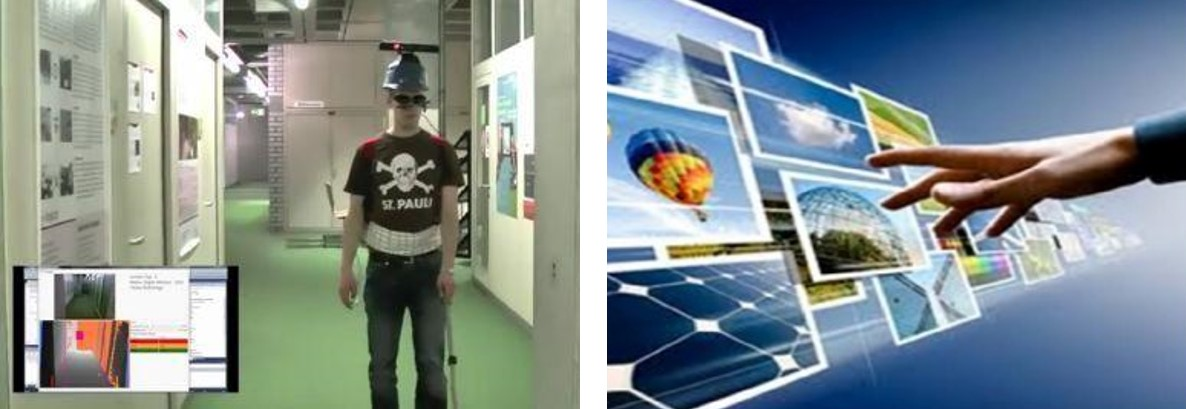
\includegraphics[width=\textwidth]{./figures/c1_apply_1.jpg}
    \begin{minipage}[t]{0.48\linewidth}
    \centerline{ \small (a) 盲人辅助设备}
    \end{minipage}
    \begin{minipage}[t]{0.48\linewidth}
    \centerline{ \small (b) 基于内容的海量图像检索}
    \end{minipage}
    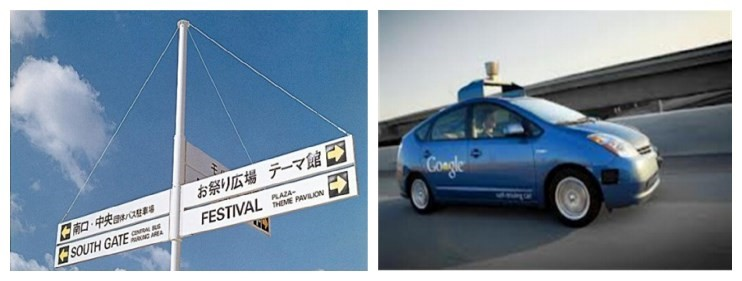
\includegraphics[width=\textwidth]{./figures/c1_apply_2.jpg}
    \begin{minipage}[t]{0.48\linewidth}
    \centerline{ \small (d) 国外旅游辅助}
    \end{minipage}
    \begin{minipage}[t]{0.48\linewidth}
    \centerline{ \small (e) 无人驾驶导航系统}
    \end{minipage}
    \caption{自然场景中文字检测与识别的应用}
    \label{fig.c1_apply}
    \end{figure*}

    在图像信息检索方面,通过计算机自动获取图像中可能存在的文字信息,可帮助计算机理解图像内容,实现对图像的自动标注,从而辅助图像搜索引擎,视频网站等工程场景的建设;在文档图像处理系统方面,可应用于淘宝、大众点评等门户网站,通过对顾客或商家上传的大量图像文件如发票、许可证书等进行文字检测和识别,可对图像进行自动判别和归类,以取代耗时耗力的人工审核;无人驾驶导航系统需要从无人驾驶汽车所处的道路环境中收集有效信息,并规划出从起点到终点的最优路径,而检测及提取出道路上标识牌中的文字信息,往往是无人驾驶导航系统能够安全、合法地行驶的必要条件;盲人辅助系统同样可通过文字检测获取标识牌及周围环境的文字信息,并通过文字识别将文字信息转换为语音或其它行驶的信息来辅助盲人获取环境信息。

    文字检测根据文字的存储媒介的不同又可分为不同类型如视频文字检测,自然场景图像文字检测等。其中,自然场景图像是指由人工拍摄而非计算机直接生成的图像。自然场景中拍摄的图像,其图像质量易受拍摄环境及拍摄条件的影响,背景较为复杂,图像中文字的字体、颜色及形态多变,这些因素都使得自然场景图像中的文字检测较为困难,呈现如图 \ref{fig.c1_problem} 所示的一些需要解决的难题:

    \begin{figure*}[!h]
    \centering
    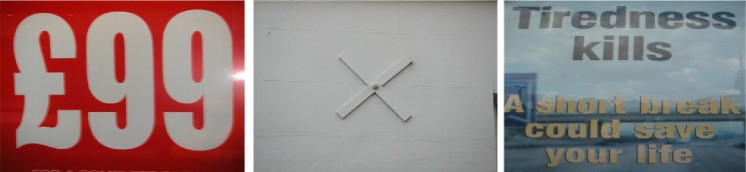
\includegraphics[width=\textwidth]{./figures/c1_problem_1.jpg}
    \begin{minipage}[t]{0.31\linewidth}
    \centerline{ \small (a) 多尺度}
    \end{minipage}
    \begin{minipage}[t]{0.31\linewidth}
    \centerline{ \small (b) 对比度低}
    \end{minipage}
    \begin{minipage}[t]{0.31\linewidth}
    \centerline{ \small (c) 不同颜色}
    \end{minipage}
    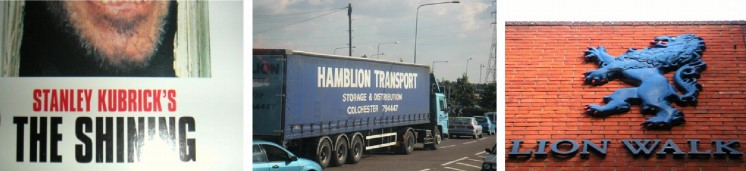
\includegraphics[width=\textwidth]{./figures/c1_problem_2.jpg}
    \begin{minipage}[t]{0.31\linewidth}
    \centerline{ \small (d) 不均匀光照}
    \end{minipage}
    \begin{minipage}[t]{0.31\linewidth}
    \centerline{ \small (e) 排列方向多变}
    \end{minipage}
    \begin{minipage}[t]{0.31\linewidth}
    \centerline{ \small (f) 复杂背景}
    \end{minipage}
    \caption{自然场景文字领域的挑战}
    \label{fig.c1_problem}
    \end{figure*}

    这些挑战包括:复杂的自然场景:在自然环境中,有许多类似文字的人为目标,例如建筑、标志和绘画等。复杂的自然场景使得文字难以从背景中被区分开来;对比度过低:文字通常与背景有一定的对比度以便于人类识别。但是某些时候,文字可能与背景有非常相似的纹理和颜色,这时文字就难以被分辨出来;不均匀的光照:由于图像采集时的光照影响和图像采集设备的不均匀响应,会使图像中产生不均匀的光照,有时图像过暗,有时图像局部太亮。不均匀光照会引入颜色失真和恶化的视觉特征,从而导致错误的分割和检测结果;排列方向多变 自然场景图像中的文字不仅是水平或竖直排列,也会倾斜排列或者曲线排列。不同的排列方向使得文字检测需要考虑更多情况从而变得困难;多语种:世界上的语种数量较多,常见的有英文、中文、日文、阿拉伯文等。不同语种的文字有不同的特点,使得在进行文字检测识别时需要考虑很多不同情况。在自然场景中进行多语种文字检测识别是非常困难的;图像模糊和退化:由于图像采集时多变的工作条件和自动对焦的使用,散焦和模糊的自然图像时常会产生。图像压缩和解压也会影响图像的质量,特别是图像中的文字。图像散焦、模糊和退化会降低文字的锐度使得文字粘连在一起,使得文字分割检测变得更加困难;图像失真:当图像采集时图像采集设备如相机等的光轴不垂直于文字所在平面时会产生透视变形。文字包围盒不是矩形和字符扭曲,都会使失真的文字难以被检测出来。

    近年来在文字检测与识别领域,研究者们为解决上述难题做了大量的研究和探索,提出了大量的文字检测方法,检测结果也在逐年提高。但目前的方法在ICDAR公开测试集上的测评结果表明,自然场景图像中的文字检测和识别效果仍有提升空间。

    \section{国内外研究现状}
    \esection{Related Work}
    
    自然场景图像中的文字检测和识别是计算机视觉领域的研究热点,国内外的很多学者在从事该方面的研究,他们也提出了很多的方法来解决这个问题,而Ye 等人\cite{Ye2015Text}对这些方法进行了调研和总结。 同时,在国际会议ICDAR 上举办了多次关于文字检测的比赛“Robust Reading”\cite{Karatzas2013ICDAR},自然场景中的文字检测及识别就是其中的一项比赛内容,不仅为从事文字检测方面研究的人提供了交流的机会,而且也反映了当时文字检测的最先进水平。
    
    自然场景图像中的文字检测方法按照其处理对象的不同,可分为基于纹理的方法和基于区域的方法:基于纹理的文字检测方法,把文字当作一种特殊纹理,通常通过局部颜色对比度、笔划滤波器、频域变换等方法来刻画文字的纹理特征。在确定纹理特征提取方式之后,往往会使用各种分类模型训练文字-背景分类器,以滑动窗的形式判断图像局部区域内是否包含文字,由此生成文字概率图。之后通过聚类或图像分割等方法取得候选文字行或文字区域,再经过后处理生成最终的检测结果。为检测不同尺寸的文字,基于纹理的方法往往需要在输入图像的不同尺度的图像上都进行同样的纹理特征提取和区域分类,或设计不同大小的纹理特征提取模板在同一个滑动窗内提取多次特征,并进行多尺度的结果融合。因此这类方法比较耗时;基于区域的文字检测方法,通常利用文字具有与背景差异明显且均一的颜色这一特征,从输入图像中提取出有限个数的候选文字区域,然后使用一些经验性的规则,或者提取区域的几何、纹理等特征,使用分类模型来滤除掉背景区域。基于区域的方法通常要比基于纹理的方法效率更高,因为基于区域的方法需要处理的区域数目有限。但这类方法的缺点在于,文字区域由于光照、遮挡、模糊等原因,内部颜色分布差异变大,或者边缘模糊,往往会在提取候选文字区域时被漏检,会直接影响最终检测结果。
    
    2010年,Epshtein\cite{Epshtein2010Detecting}等人提出了笔画宽度变换(SWT)来计算图像中每个像素的笔画,基于像素笔画产生候选文字连通区域,去掉非文字连通区域就得到文字检测结果。笔画是组成文字的基本元素,通过计算笔画来检测文字是文字检测中非常有意义的研究进展;2011年,Neumann和Matas\cite{Neumann2011Text} 使用最稳定极值区域(MSER)作为候选文字区域,通过有效剪枝可以详尽搜索所有可能文字序列,并利用高阶文字属性(文字行)对候选区域进行区分从而确定文字区域;2012 年,Tu\cite{Tu2012Detecting}等提出了一种检测自然图像中任意方向的文字的方法,他们使用SWT来获得候选文字连通区域,然后通过单个连通区域的分析和连通区域行的分析来去掉非文字部分,保留下来的连通区域就是文字检测的结果;2014年,Yin\cite{Yin2013Robust}等设计了一个快速有效的剪枝算法来提取图像中的最稳定机制区域(MSER)作为候选文字连通区域,他们通过一个单链聚类算法将候选文字链接成候选文字行,这个聚类算法的距离权重和聚类阈值是通过一个自训练距离度量学习算法自动学习到的,通过贝叶斯模型利用字符分类器计算候选文字的后验概率,从而将文字检测出来;2015年,Yu\cite{Yu2015Text} 等提出了一种基于边缘分析的文字检测方法,他们使用边缘重组来产生候选文字连通区域,然后通过单个连通区域分析、连通区域行分析对候选文字进行验证,得到最终的文字检测结果。
    
    近些年,随着深度学习\cite{Moral2010Foundations}的兴起,它被广泛用于目标检测识别任务,例如手写字符识别、交通标志识别等,同时取得了非常好的结果,大大提升了目标检测识别的水平。鉴于深度学习的良好表现,许多人也将深度学习用于自然场景中的文字检测。

    \section{本文研究内容}
    \esection{Research Contents}

    \section{论文的组织结构}
    \esection{Thesis Structure}


